\documentclass[8pt]{beamer}
\usepackage[utf8]{inputenc}
\usepackage{xcolor}
\usepackage{colortbl}
\usepackage{epsfig}
% \usepackage{cancel}
\usepackage{ulem}
% \usepackage{threeparttable} % Joao Pela: 
\usepackage{amsmath}
\usepackage{hyperref}
\usepackage{siunitx}  % Allows easy x10^ for numbers
\usepackage{appendixnumberbeamer}

\usetheme{Madrid}

\author[J. Pela]{João Pela}
\title{QCD VBFMET Gridpack Validation}
\institute[ICL]{Imperial College London}
\date{2015-11-09}

% The log drawn in the upper right corner.
\logo{\includegraphics[height=0.115\paperheight]{img/Logo_CMSICL.png}}

\begin{document}
\setlength{\unitlength}{1mm}


% ###################################################
\begin{frame}
  \titlepage
\end{frame}


% ###################################################
\begin{frame}{MadGraph Gridpack v2 characteristics}
  
\begin{itemize}
  \item A grid pack was generated following the instructions found in the TWiki below:
   \begin{itemize}
     \item \href{https://twiki.cern.ch/twiki/bin/viewauth/CMS/QuickGuideMadGraph5aMCatNLO}{TWiki: QuickGuideMadGraph5aMCatNLO}
   \end{itemize}
  \item Patches to include custom cuts were produced and included in the gridpack generation code
  \item Include optimizations recommend by Josh Bendavid
\end{itemize}

\begin{block}{Sample characteristics}

\begin{itemize}
  \item Process: $pp \rightarrow jj,jjj,jjjj$
  \item At least one dijet with:
  \begin{itemize}
    \item Jets $p_\perp > 30$ $GeV$
    \item Dijet $m_{jj} > 800$ $GeV$
  \end{itemize}
\end{itemize}

\end{block}

\begin{block}{What changed from previous studies:}

\begin{itemize}
  \item Different MAdGraph version: MG5\_aMC\_v2\_3\_0  $\rightarrow$ MG5\_aMC\_v2.3.2.2 
  \item Additional CMS patches and options
  \begin{itemize}
    \item Physics Model: sm $\rightarrow$ sm-ckm\_no\_b\_mass
    \item PDF choice: nn23lo1 $\rightarrow$ lhapdf(263000)
    \item Remove jet min $p_\perp$ and added auto jet $p_\perp$ and $m_{jj}$ optimization option
  \end{itemize}
\end{itemize}

\end{block}

\end{frame}

% ###################################################
\begin{frame}{Hadronization}

\begin{block}{Software}

  \begin{itemize}
    \item Using CMSSW\_7\_1\_19 (\textbf{NEW:} before was CMSSW\_7\_1\_18. Changed to match MG production version.)
    \item Showering: Pythia8
    \item Hadronizer: \tiny{Configuration/Generator/python/Hadronizer\_TuneCUETP8M1\_13TeV\_MLM\_5f\_max4j\_LHE\_pythia8\_cff.py}
  \end{itemize}

\end{block}

\begin{block}{Results}

\resizebox{1.0\textwidth}{!}{
\begin{tabular}{|c|c|c|c|c|c|}
\hline
                          & \multicolumn{3}{c|}{Events}      & \multicolumn{2}{c|}{Cross Section [pb]}                                       \\
\hline
Process                   & Tried  & Passed & accepted [\%]  & Before                                & After                                 \\
\hline\hline 
$p p \rightarrow j j$     &  53110 &  12392 & $23.3 \pm 0.2$ & $\num{1.652e+06} \pm \num{9.011e+03}$ & $\num{3.854e+05} \pm \num{3.689e+03}$ \\
$p p \rightarrow j j j$   & 114701 &   8253 & $ 7.2 \pm 0.1$ & $\num{3.629e+06} \pm \num{1.980e+04}$ & $\num{2.611e+05} \pm \num{3.114e+03}$ \\
$p p \rightarrow j j j j$ & 157189 &  10054 & $ 6.4 \pm 0.1$ & $\num{4.962e+06} \pm \num{2.707e+04}$ & $\num{3.174e+05} \pm \num{3.518e+03}$ \\
\hline\hline
Total                     & 325000 &  30699 & $ 9.4 \pm 0.1$ & $\num{1.024e+07} \pm \num{3.473e+04}$ & $\num{9.638e+05} \pm \num{5.973e+03}$ \\
\hline
\end{tabular}
}



\end{block}

\begin{itemize}
  \item[] \textbf{The 3 and 4 jets configurations fail more events since there is no restriction on min(jet $p_\perp$) which fails sometime the imposed hadronizer cut.}
  \item[] \textbf{Values are almost the same as gridpack v1 only small changes observed.}
\end{itemize}

\end{frame}

% ###################################################
\begin{frame}{Selected Di-parton I}

\begin{columns}

  \column[t]{0.45\linewidth}  
  \centering

  \begin{block}{Lead Parton $p_\perp$}
    \centering
    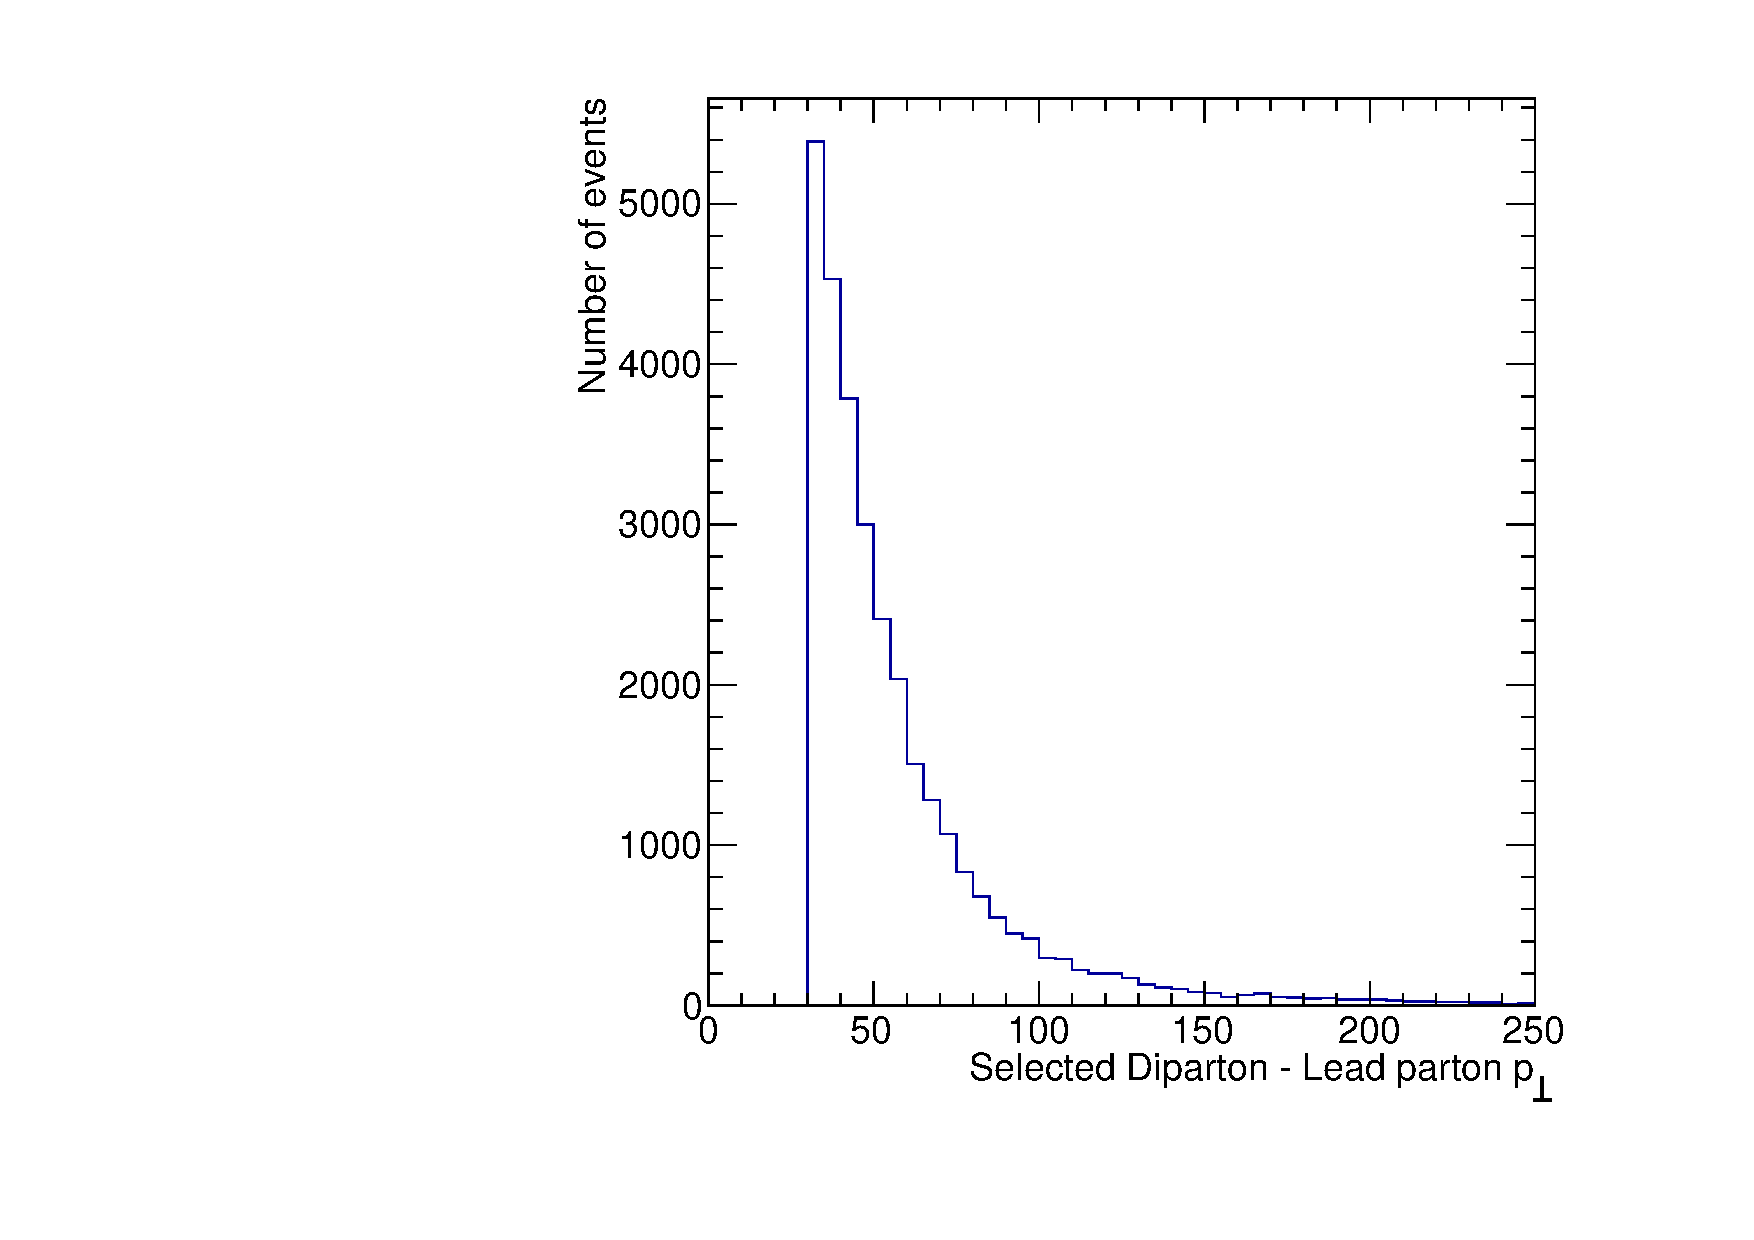
\includegraphics[width=0.8\linewidth]{img/SelDiParton_Parton1_Pt.pdf}
  \end{block}
  
  \column[t]{0.45\linewidth}  
  \centering

  \begin{block}{Sublead Parton $p_\perp$}
    \centering
    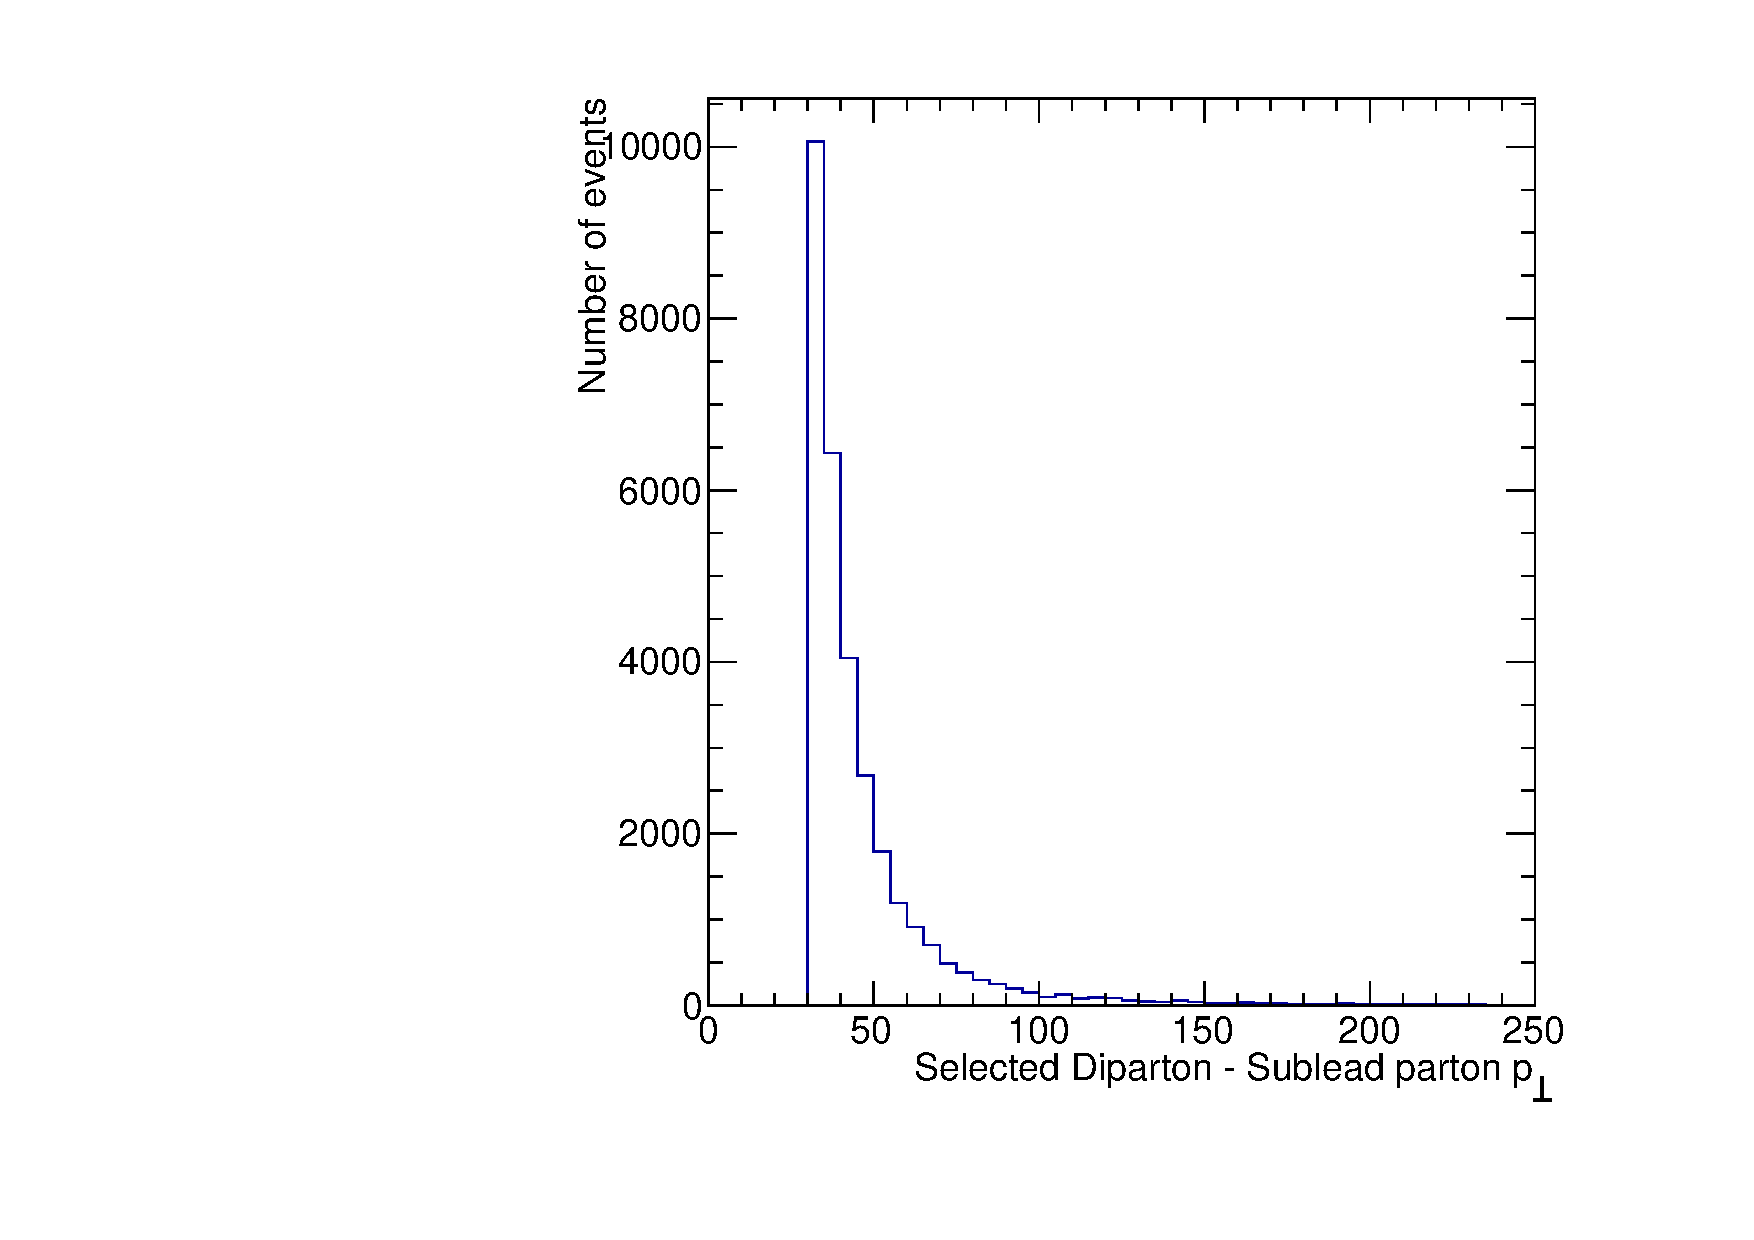
\includegraphics[width=0.8\linewidth]{img/SelDiParton_Parton2_Pt.pdf}
  \end{block}

\end{columns}

\begin{center}
\textbf{Custom MadGraph cuts on dijet parton $p_\perp$ are implemented correctly.}
\end{center}

\end{frame}

% ###################################################
\begin{frame}{Selected Di-parton II}

\begin{columns}

  \column[t]{0.45\linewidth}  
  \centering

  \begin{block}{Lead Parton $p\eta$}
    \centering
    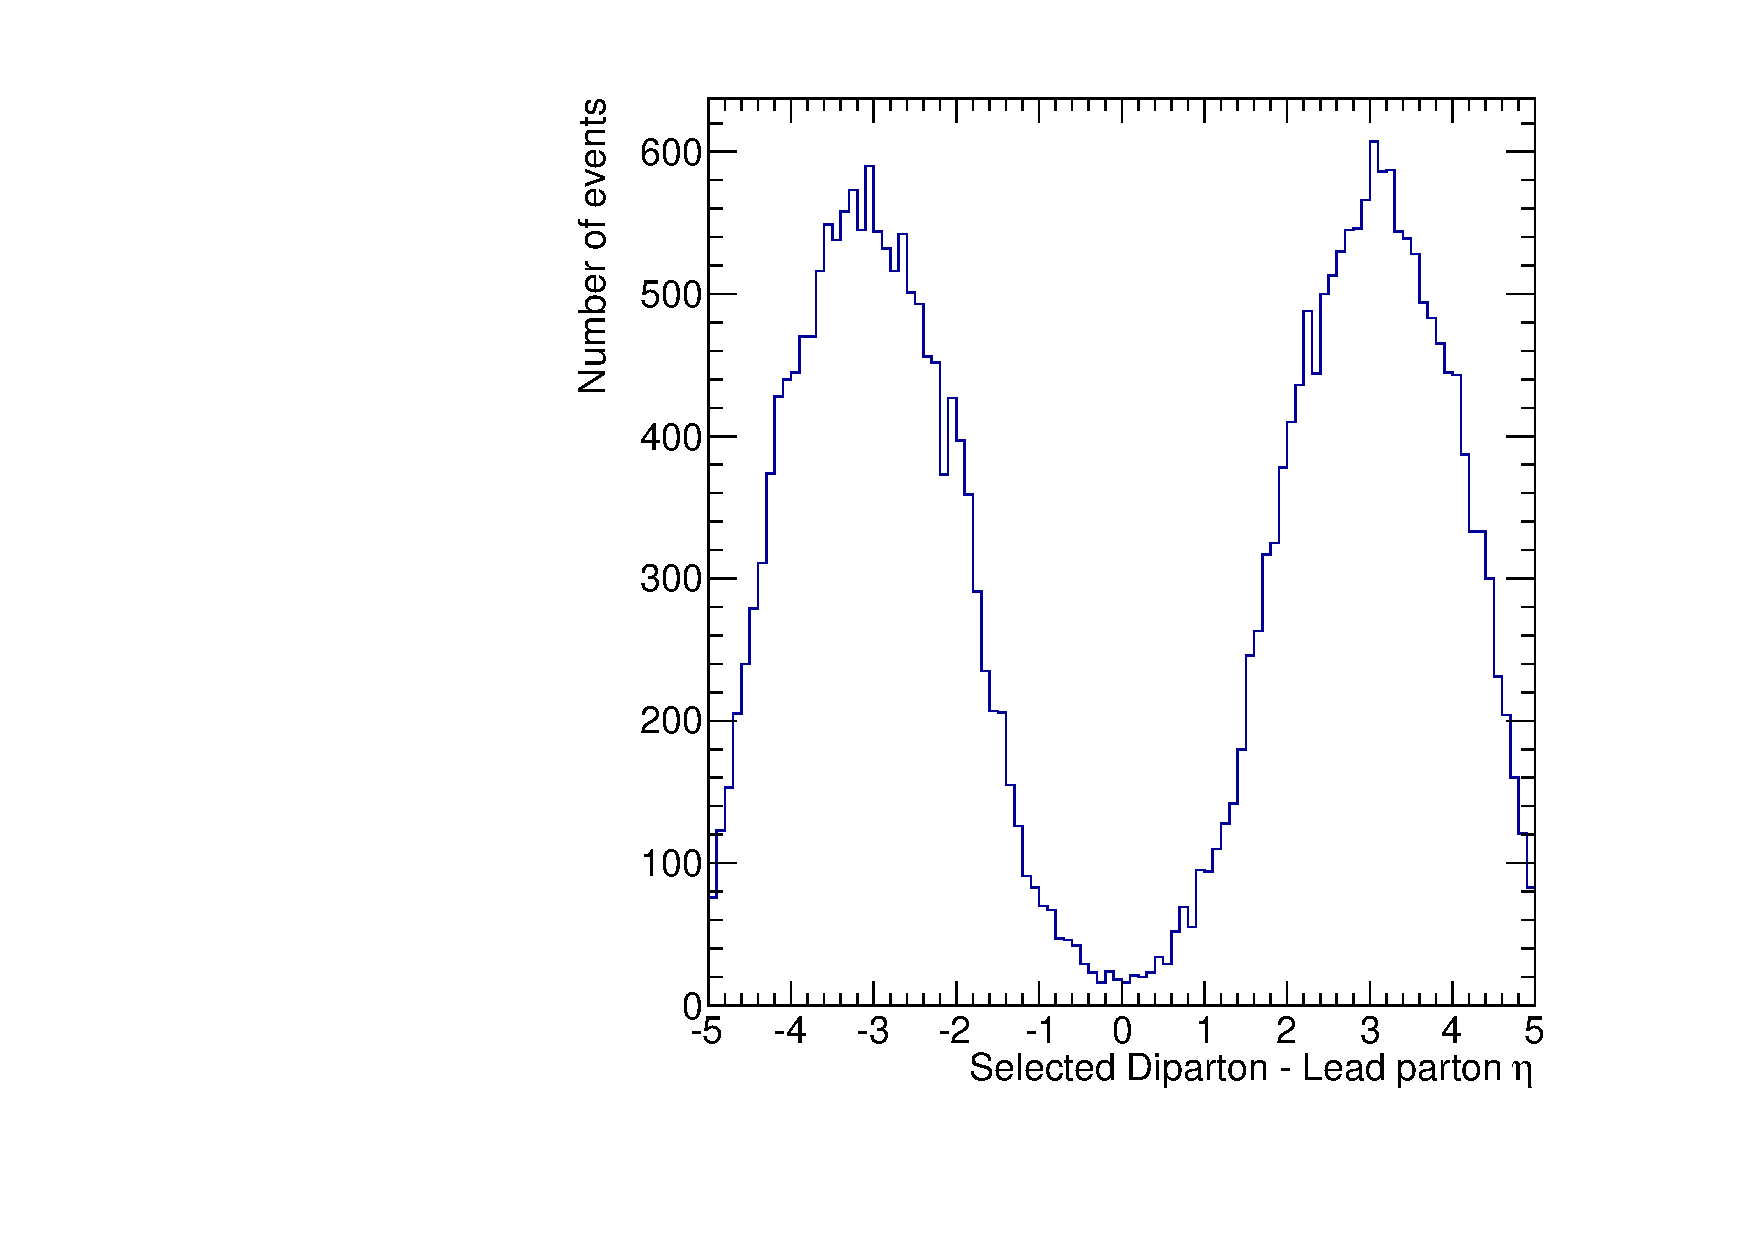
\includegraphics[width=0.8\linewidth]{img/SelDiParton_Parton1_Eta.pdf}
  \end{block}
  
  \column[t]{0.45\linewidth}  
  \centering
 
  \begin{block}{Sublead Parton $\eta$}
    \centering
    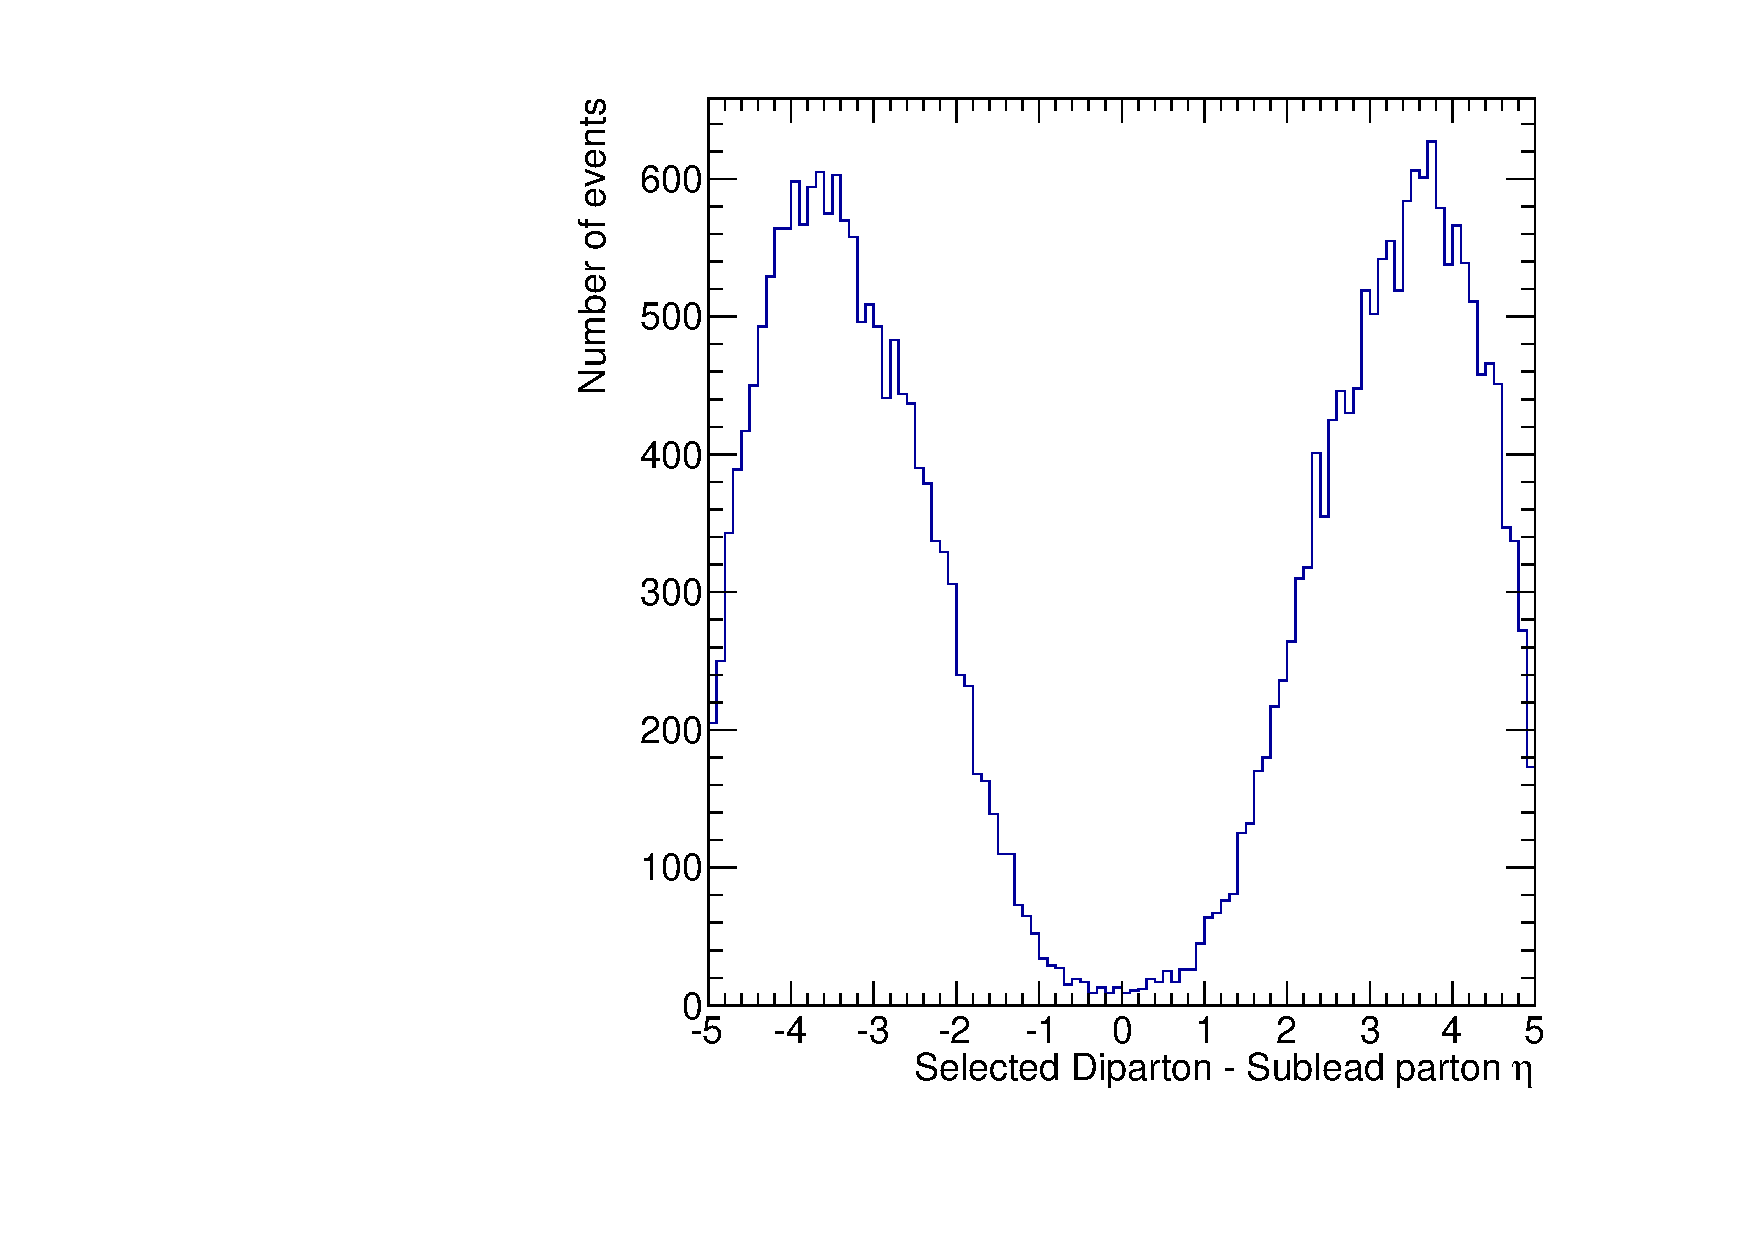
\includegraphics[width=0.8\linewidth]{img/SelDiParton_Parton2_Eta.pdf}
  \end{block}

\end{columns}

\begin{center}
\textbf{Jet $\eta$ distribution looks ok. MadGraph cut is at 5.0.}
\end{center}

\end{frame}

% ###################################################
\begin{frame}{Selected Di-parton III}

\begin{columns}

  \column[t]{0.45\linewidth}  
  \centering

  \begin{block}{Di-parton $\Delta\eta$}
    \centering
    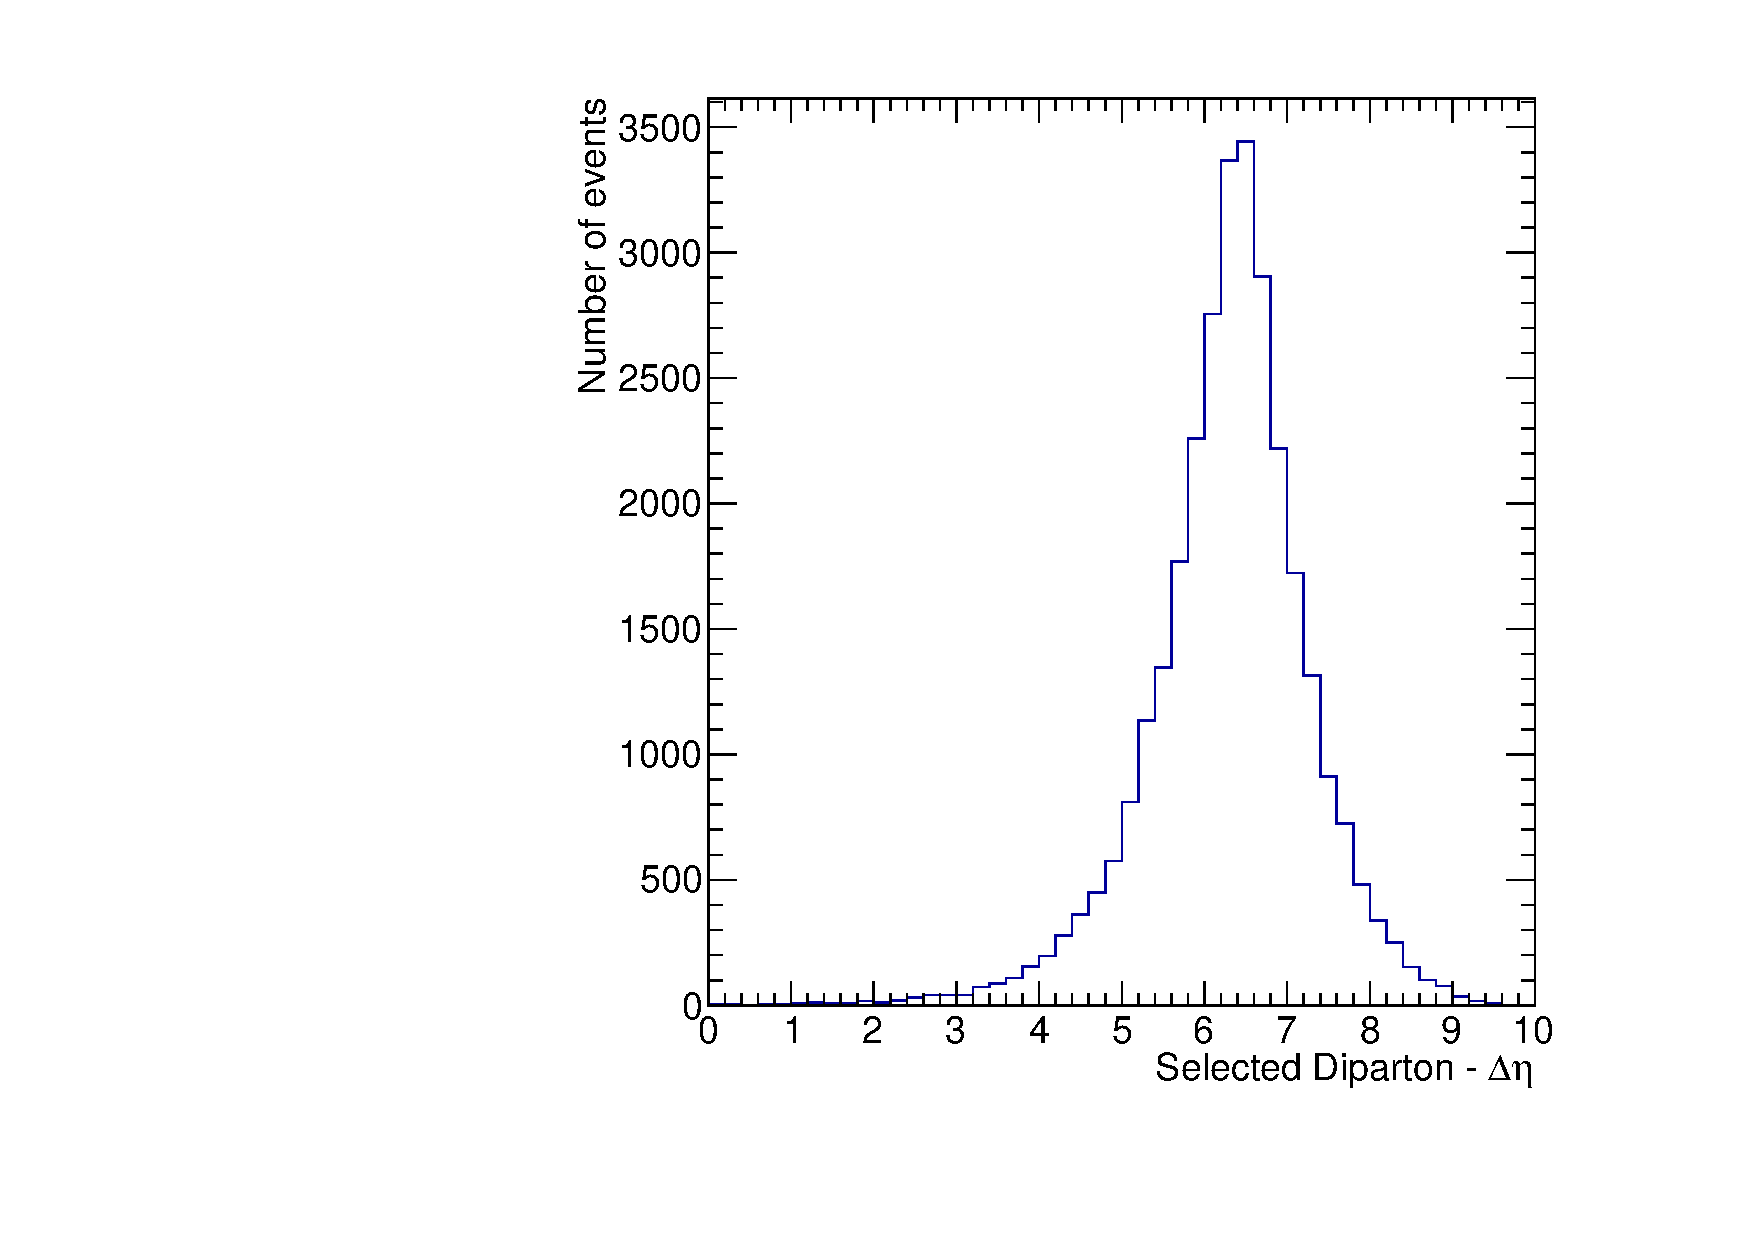
\includegraphics[width=0.8\linewidth]{img/SelDiParton_DEta.pdf}
  \end{block}
  
  \column[t]{0.45\linewidth}  
  \centering
 
  \begin{block}{Di-parton $m_{jj}$}
    \centering
    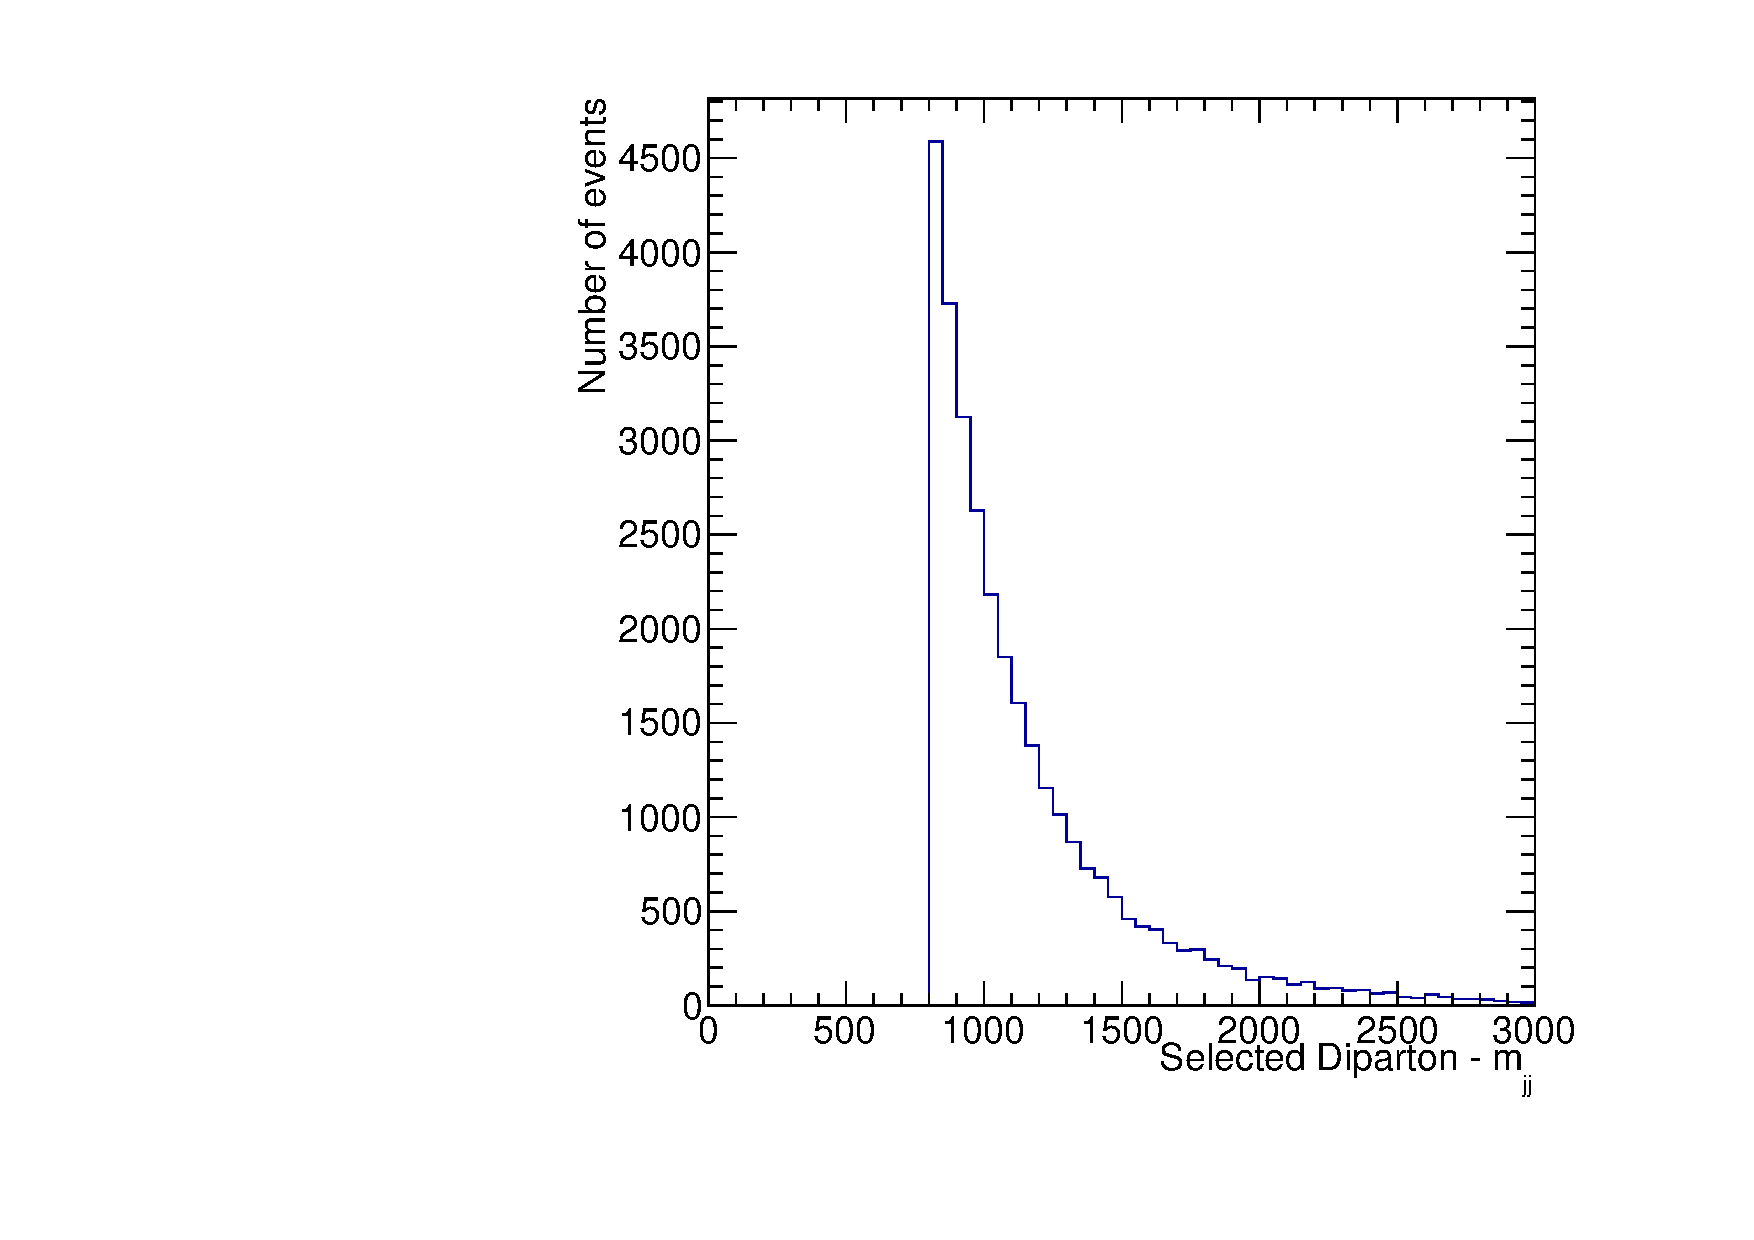
\includegraphics[width=0.8\linewidth]{img/SelDiParton_Mjj.pdf}
  \end{block}

\end{columns}

\begin{center}
\textbf{Custom MadGraph cuts on dijet parton $m_{jj}$ are implemented correctly. $\Delta\eta$ peaks over 6 showing that this variable indeed could not be used to reduce QCD.}
\end{center}

\end{frame}

% ###################################################
\begin{frame}{Parton-Generator Jet Matching procedure}

\begin{block}{Pairing Partons and Generator Jets}

\begin{itemize}
  \item Selecting all generator jets within $\Delta R < 0.4$ 
  \item From those selecting the generator jet with the lowest $p_\perp$ to the parton as a match.
  \begin{itemize}
    \item This avoids picking up the wrong jet from just picking lowest $\Delta R$
  \end{itemize}
\end{itemize}

\end{block}

\begin{block}{Results}
  
\begin{center}

\begin{tabular}{|c||c|c|c||c|}
\hline
            &          \multicolumn{4}{c|}{Process} \\
\hline
$n_{match}$ &      jj &    jjj  &    jjjj &   Total \\
\hline\hline 
          0 &  3.42\% &  0.30\% &  0.08\% &  1.49\% \\
          1 & 25.27\% &  4.79\% &  1.02\% & 11.82\% \\
          2 & 71.30\% & 28.29\% &  8.89\% & 39.30\% \\
          3 &         & 66.61\% & 36.36\% & 29.82\% \\
          4 &         &         & 53.64\% & 17.57\% \\
\hline
\end{tabular}

\end{center}

\begin{itemize}
  \item Selected diparton has a match     : 73.12\%
  \item Generator jet matched not lowest $\Delta R$ :  3.52\%
\end{itemize}

\end{block}

\begin{itemize}
  \item[] \textbf{With the current matching procedure we can find matches for the selected di-parton most of the times.}
  \item[] \textbf{All values are compatible with gridpack v1 (to the 1\% level)}
\end{itemize}


\end{frame}

% ###################################################
\begin{frame}{Migration study I}

A second grid pack was create with reduced thresholds to study migrations.

\begin{block}{Sample characteristics}

\begin{itemize}
  \item Process: $pp \rightarrow jj,jjj,jjjj$
  \item At least one dijet with:
  \begin{itemize}
    \item Jets $p_\perp > 10$ $GeV$
    \item Dijet $m_{jj} > 600$ $GeV$
  \end{itemize}
\end{itemize}

\end{block}

\begin{block}{Key data}

\begin{itemize}
  \item Hard process cross section is $\num{1.095e+08} \pm \num{3.924e+05}$ which is 10.7 times more than for our proposed process.
  \item 1.45M events were produced at parton level to provide enough statistics to study migration of $\approx 1\%$.
  \item Hadronization was performed the same as for for v2. 
  \begin{itemize}
    \item An event efficiency of $6.7 \pm 0.5$ was observed which is $\approx 30\%$ less than v2. Probably due to lower jet cuts.
    \item The resulting post hadronization cross section of $6.647e+06 \pm 2.380e+04$ which is 6.9 higher than v2.
  \end{itemize}
\end{itemize}

\end{block}

\end{frame}

% ##################################
\begin{frame}{Migration study I}

\vspace{-17px}

\begin{columns}

  \column[t]{0.45\linewidth}  
  \centering

  \begin{block}{Lead Parton-Generator Jet $p_\perp$}
    \centering
    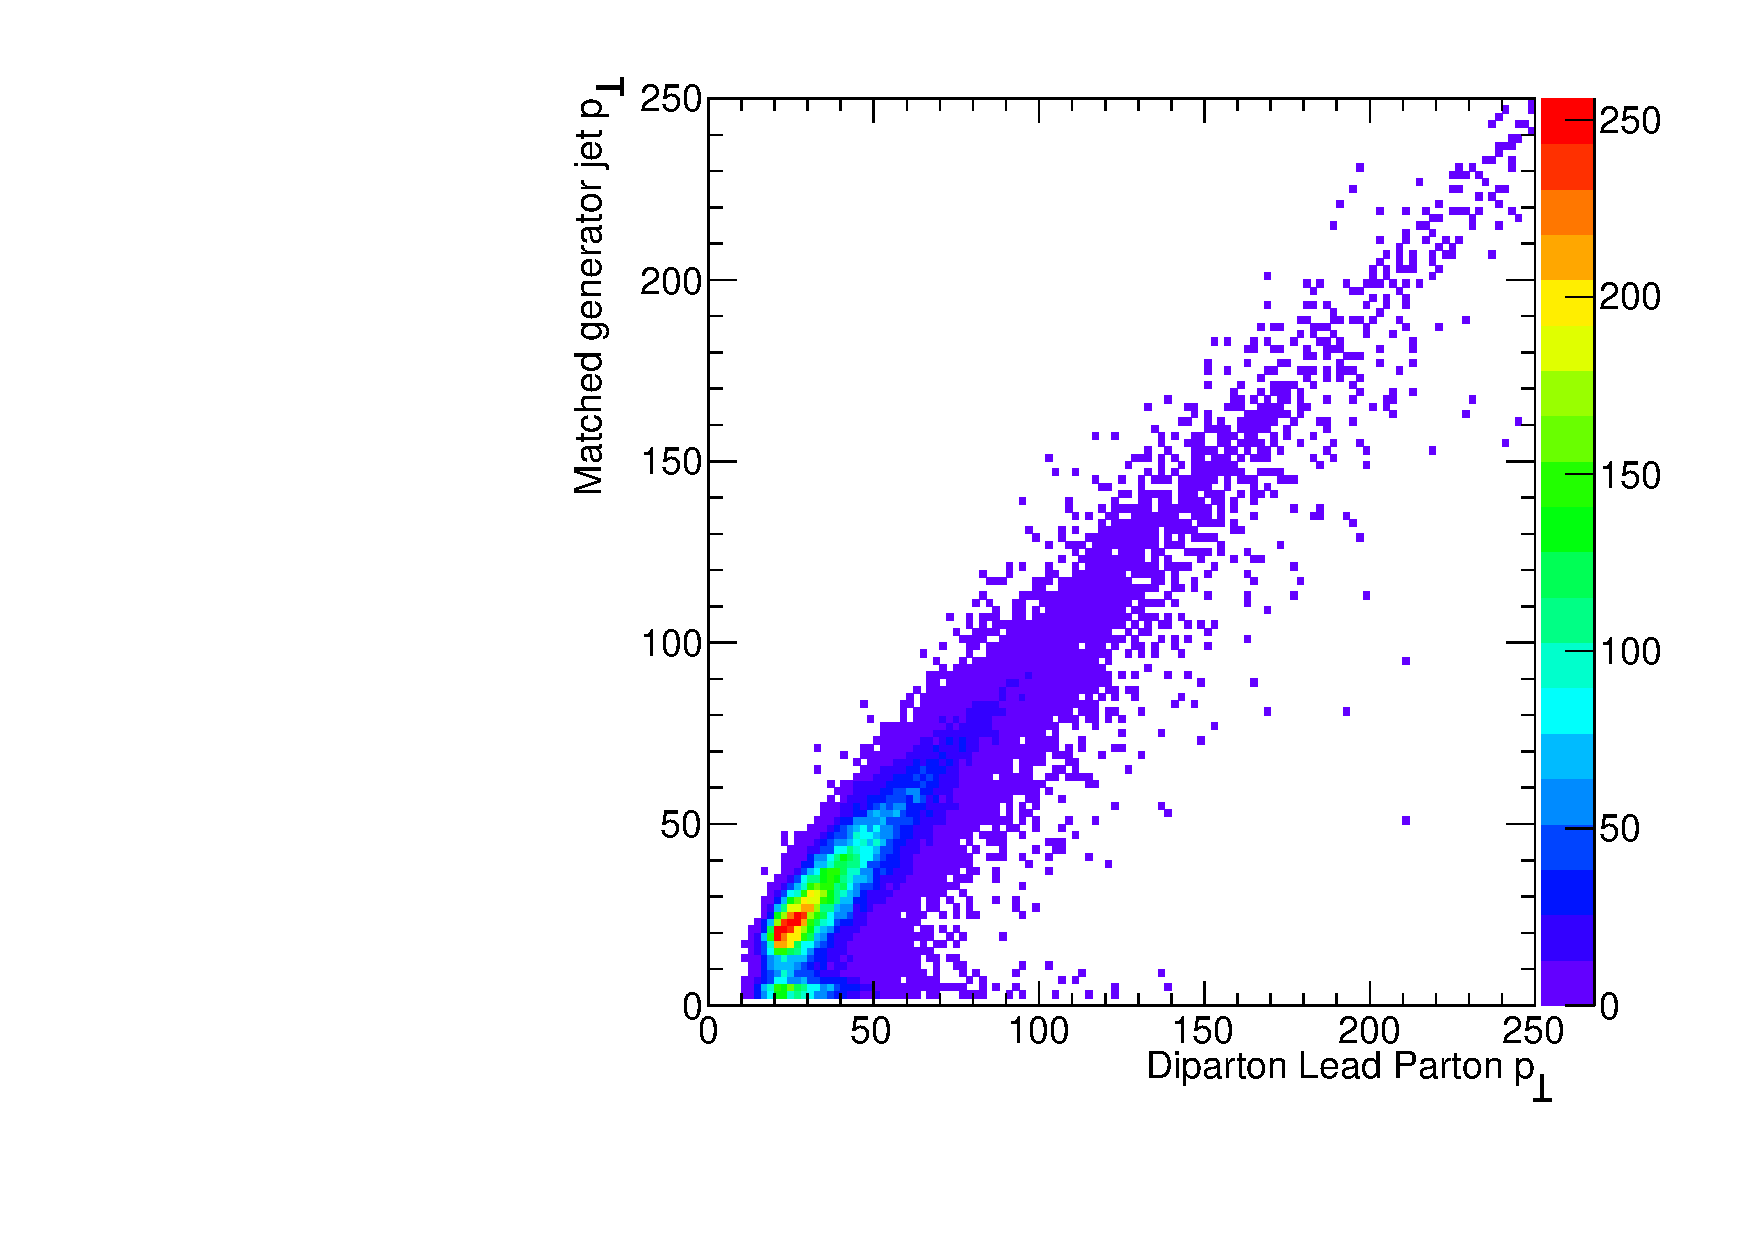
\includegraphics[width=0.8\linewidth]{img/migrations/SelDiParton_MatchedGenJet_Parton1_Pt.pdf}
    
  \end{block}
  
  \column[t]{0.45\linewidth}  
  \centering
 
  \begin{block}{Sublead Parton-Generator Jet $p_\perp$}
    \centering
    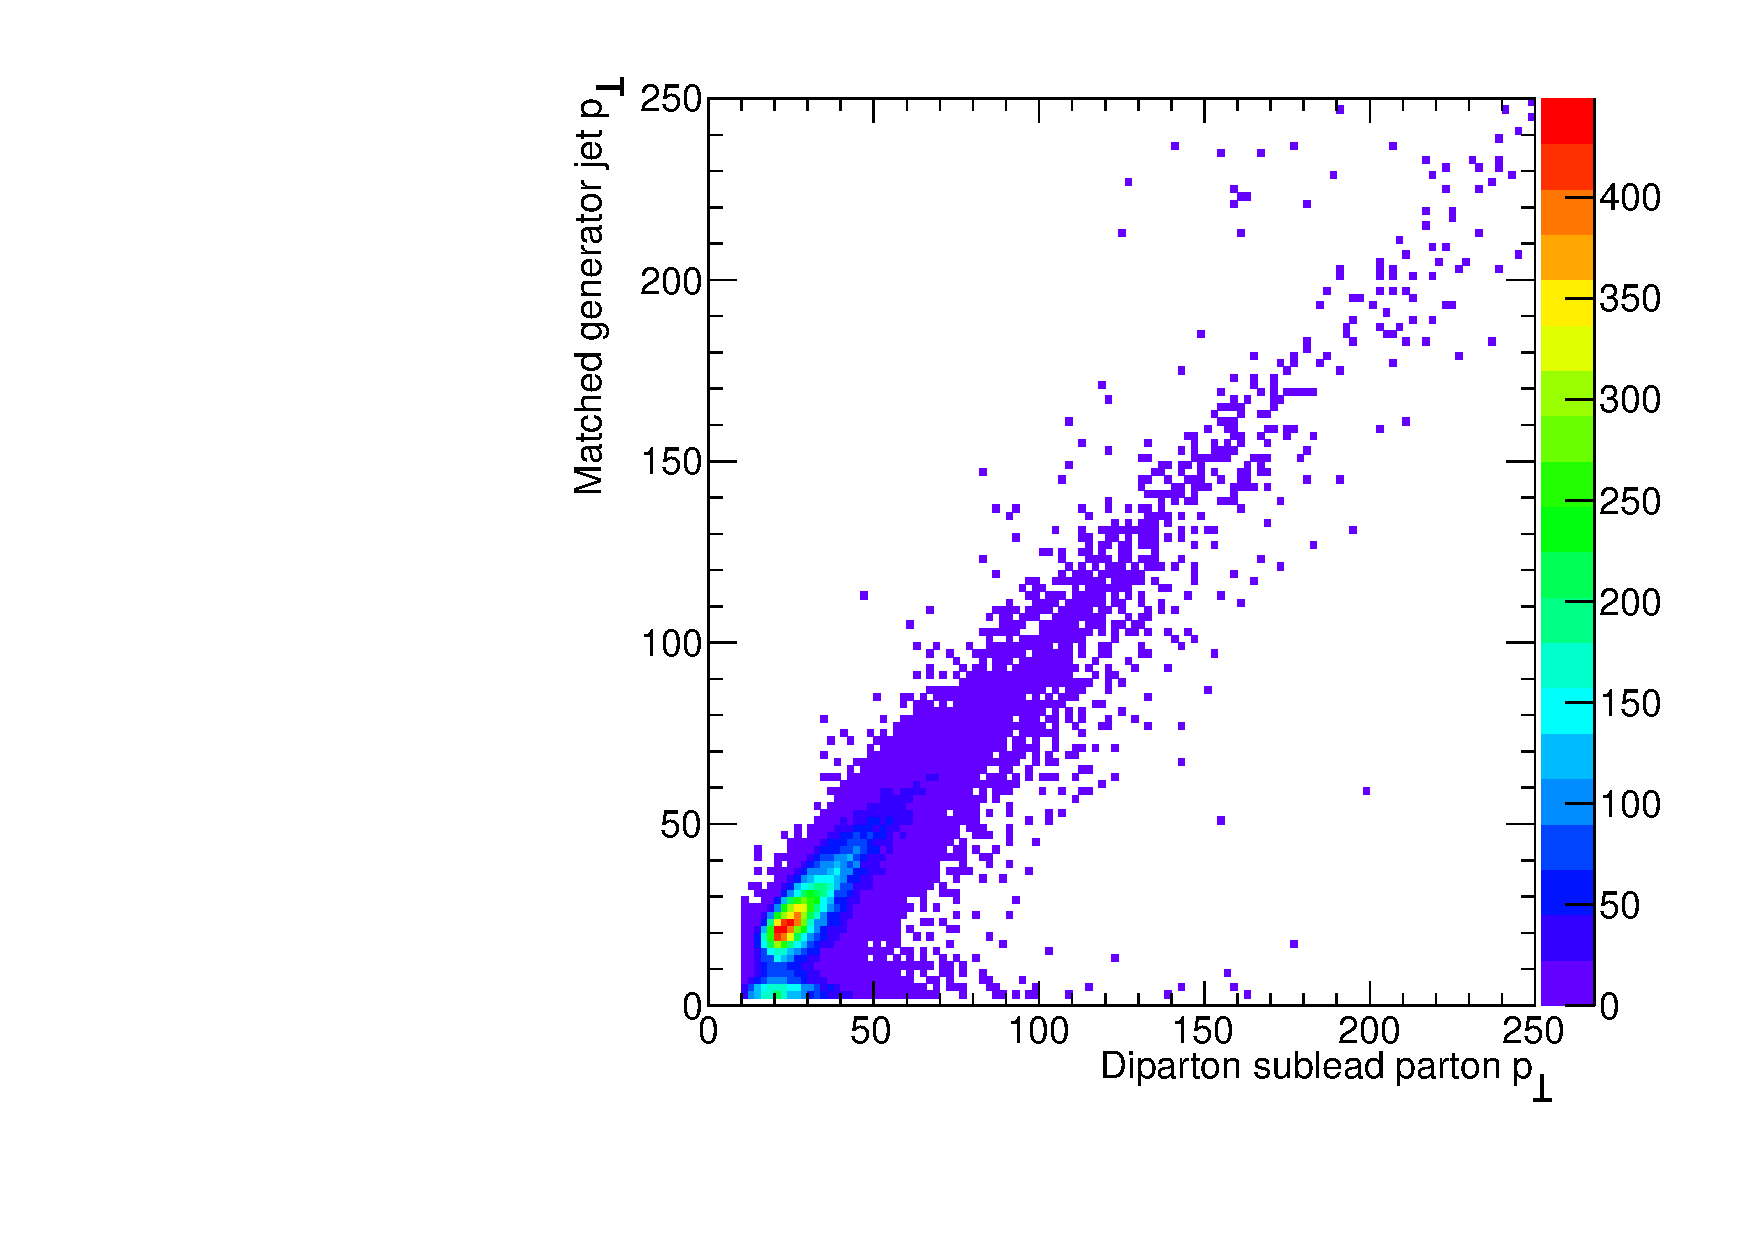
\includegraphics[width=0.8\linewidth]{img/migrations/SelDiParton_MatchedGenJet_Parton2_Pt.pdf}
  \end{block}

\end{columns}

\begin{block}{Single variable migration}
  
\begin{itemize}
  \item \tiny{Lead jets:    $\frac{p_{\perp}^{Parton}<30 \text{ AND } p_{\perp}^{GenJet} \geq 40}{p_{\perp}^{GenJet} \geq 40}=0.27\% \pm 0.04\%$  }
  \item \tiny{Sublead jets: $\frac{p_{\perp}^{Parton}<30 \text{ AND } p_{\perp}^{GenJet} \geq 40}{p_{\perp}^{GenJet} \geq 40}=0.56\% \pm 0.08\%$  }
\end{itemize}

\end{block}

\begin{center}
\textbf{Parton to generator jet $p_\perp$ migration are under 0.6\%. Much less than the 3.5\% majorated last week. This is acceptable.}
\end{center}

\end{frame}

% ###################################################
\begin{frame}{Migration study I}

\begin{columns}
  
  \column[t]{0.30\linewidth}  
  \centering
 
  \begin{block}{Parton-Generator Jet $m_{jj}$}
    \centering
    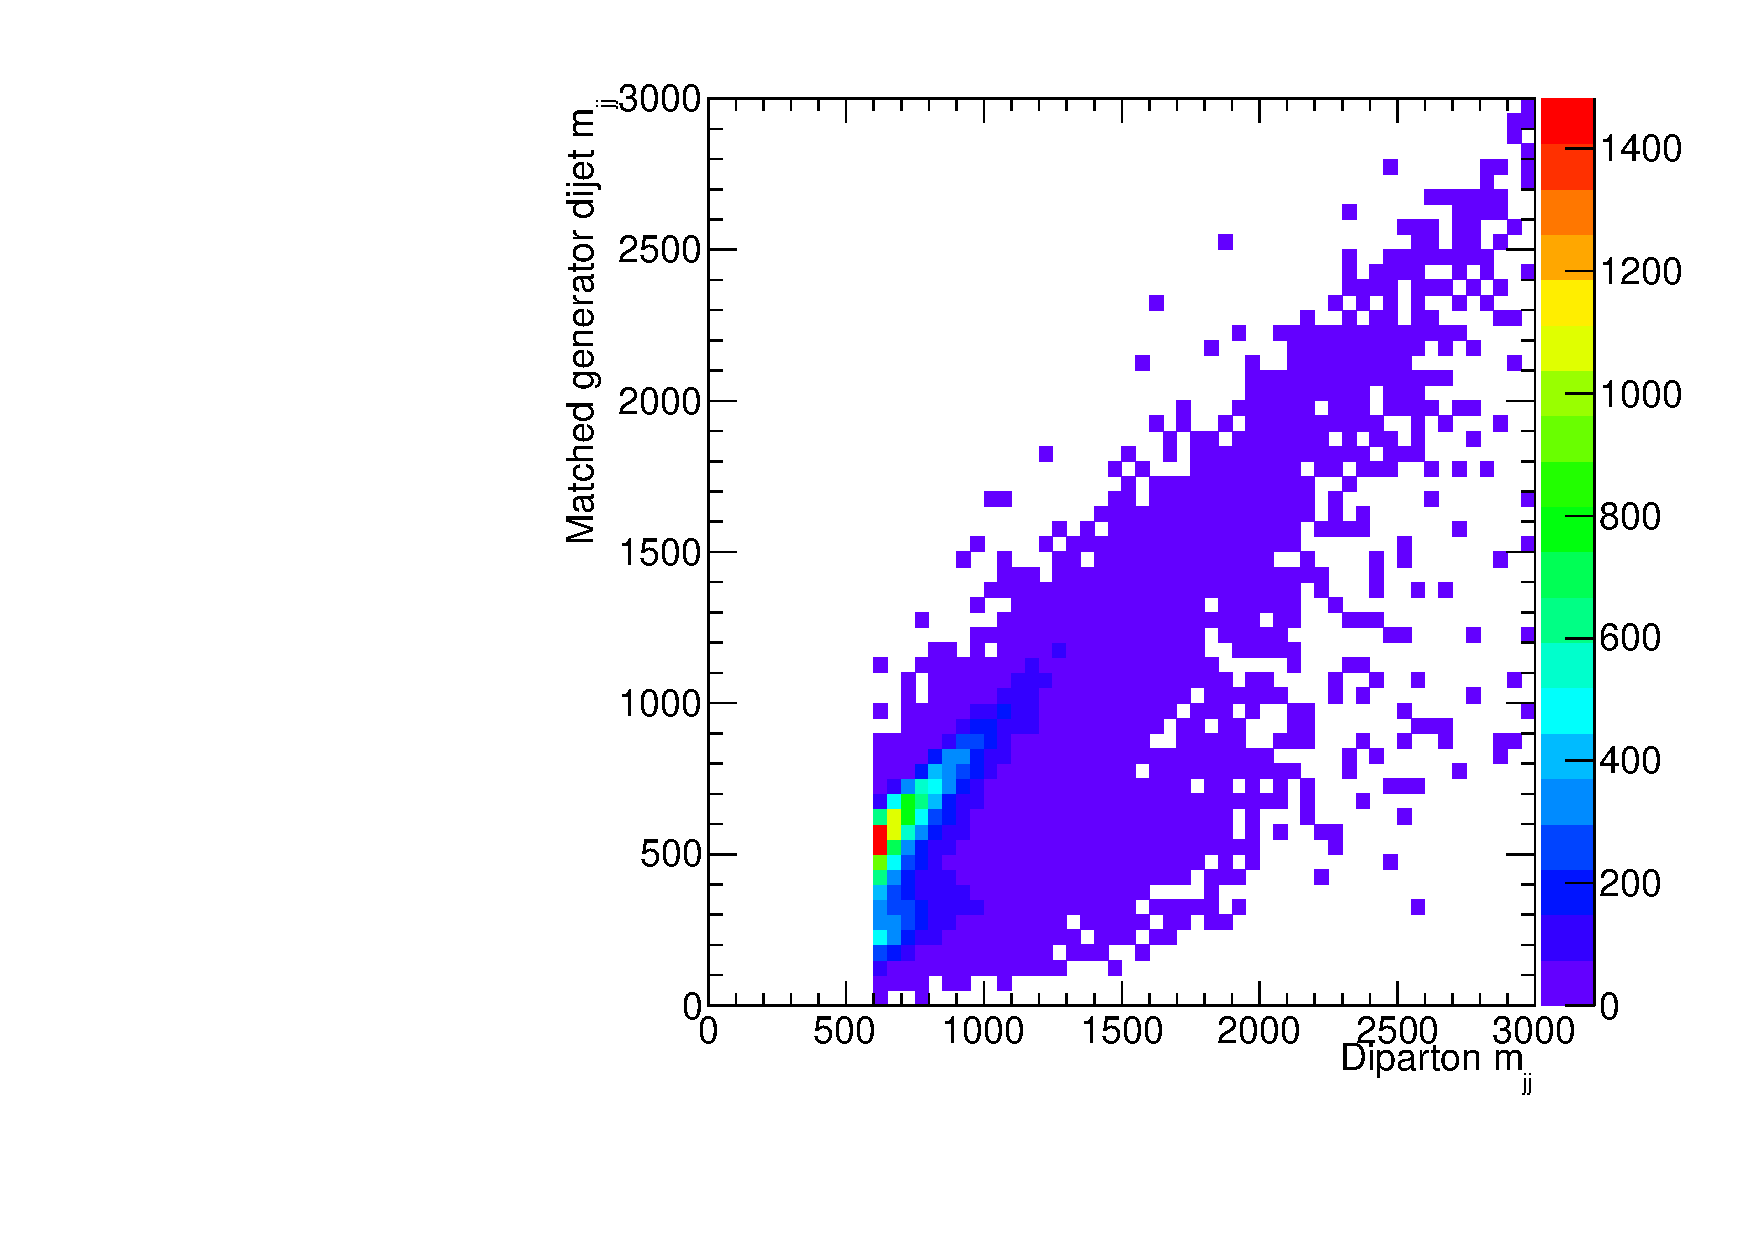
\includegraphics[width=1.0\linewidth]{img/migrations/SelDiParton_MatchedGenJet_Mjj.pdf}
  \end{block}

  \column[t]{0.67\linewidth}  
  \centering
  \begin{block}{Single variable migration}
  
    \begin{itemize}
      \item[] \tiny{Mjj: $\frac{m_{jj}^{Parton}<800 \text{ AND } m_{jj}^{GenJet} \geq 1000}{m_{jj}^{GenJet} \geq 800}=0.13\% \pm 0.04\%$  }
    \end{itemize}

  \end{block}
  
  \begin{block}{Double variable migration}
    
    \begin{itemize}
      \item \tiny{$\frac{(p_{\perp}^{GenJet}>40 \text{ AND } m_{jj}^{GenJet}>1000) \text{ AND } (p_{\perp}^{Parton}<30 \text{ OR } m_{jj}^{Parton}<800)}{p_{\perp}^{GenJet}>40 \text{ AND } m_{jj}^{GenJet}>1000} = 0.23\% \pm 0.13\%$}
    \end{itemize}

  \end{block}
  
\end{columns}

\begin{center}
\textbf{Parton to generator jet $m_{jj}$ migration are under 0.2\% and global migration are under 0.25\%. This is also acceptable.}
\end{center}

\end{frame}


% ###################################################
\begin{frame}{Conclusions}

\begin{block}{Summary}
  
\begin{itemize}
  \item A MadGraph gridpack was produce following the CMS Generator Group recommended instructions and now includes Josh Bendavid suggestions
  \begin{itemize}
    \item A test run was made producing 325k events where it was demonstrated that the custom proposed cuts were correctly implemented.
    \item Pythia8 hadronization was performed over the parton level events with an efficiency of $ 9.4 \pm 0.1$ and leading to a final sample cross section of $\num{9.638e+05} \pm \num{5.973e+03}$.
  \end{itemize}
  \item A second gridpack with lower thresholds was implemented to study variable migrations
  \begin{itemize}
    \item A test run was made producing 1.45M events with a post hadronization cross section of $\num{6.647e+06} \pm \num{2.380e+04}$ which is 6.9 times more than proposed cuts.
    \item A study over the key variable migration was performed showing that global events migration from below selected parton cuts to above selected generator cuts is of $0.23\% \pm 0.13\%$ of the total events that should pass the generator cuts. This is deemed to be acceptable.
  \end{itemize}
  \item We are ready to pass this gridpack to the generator group and request our new QCD sample production.
\end{itemize}

The gridpack and the respective cards can be found at:
\begin{center}
/afs/cern.ch/work/p/pela/public/qcd\_vbf\_samples/gridpack\_v2/
\end{center}

\end{block}

\end{frame}

\end{document}
